
%(BEGIN_QUESTION)
% Copyright 2012, Tony R. Kuphaldt, released under the Creative Commons Attribution License (v 1.0)
% This means you may do almost anything with this work of mine, so long as you give me proper credit

Examine this schematic diagram for this protective relay system, where a pair of parallel circuit breakers are controlled by two redundant overcurrent relays:

$$\includegraphics[width=15.5cm]{i02112x01.eps}$$

Identify the switch closure positions necessary to have relay \#1 control breaker \#2, and have relay \#2 control {\it both} breakers \#1 and \#2.

\vskip 10pt

Explain why the diodes are in this circuit.  Hint: these are sometimes referred to as {\it voting} diodes.  They are not used for current-measurement (as in 4-20 mA circuits), nor do they suppress transient voltages (commutating diodes across inductive loads).  

\vskip 10pt

Given a dependability value of 0.99982 for each relay and a dependability value of 0.99961 for each circuit breaker, calculate the probability that the breakers will fail to trip in an overcurrent condition with all four relay/breaker selection switches in the closed position (assume all other system components are 100\% reliable).

\vskip 20pt \vbox{\hrule \hbox{\strut \vrule{} {\bf Suggestions for Socratic discussion} \vrule} \hrule}

\begin{itemize}
\item{} A very useful problem-solving technique for figuring out the purpose of a particular device in a system is to analyze that system's behavior {\it without} the device in question.  In this example, consider how the system would function if the voting diodes were {\it not} installed in the trip circuitry.
\end{itemize}

\underbar{file i02112}
%(END_QUESTION)





%(BEGIN_ANSWER)

If not for the diodes, trip signal current would ``backfeed'' in such a way that one relay might end up tripping both circuit breakers even though you only intended it to trip one circuit breaker.

\vskip 10pt

Dependability/PFD calculation:

$$\includegraphics[width=15.5cm]{i02112x03.eps}$$

%(END_ANSWER)





%(BEGIN_NOTES)

Switch positions (\#2 through \#4 closed, \#1 open):

$$\includegraphics[width=15.5cm]{i02112x02.eps}$$

\filbreak

$$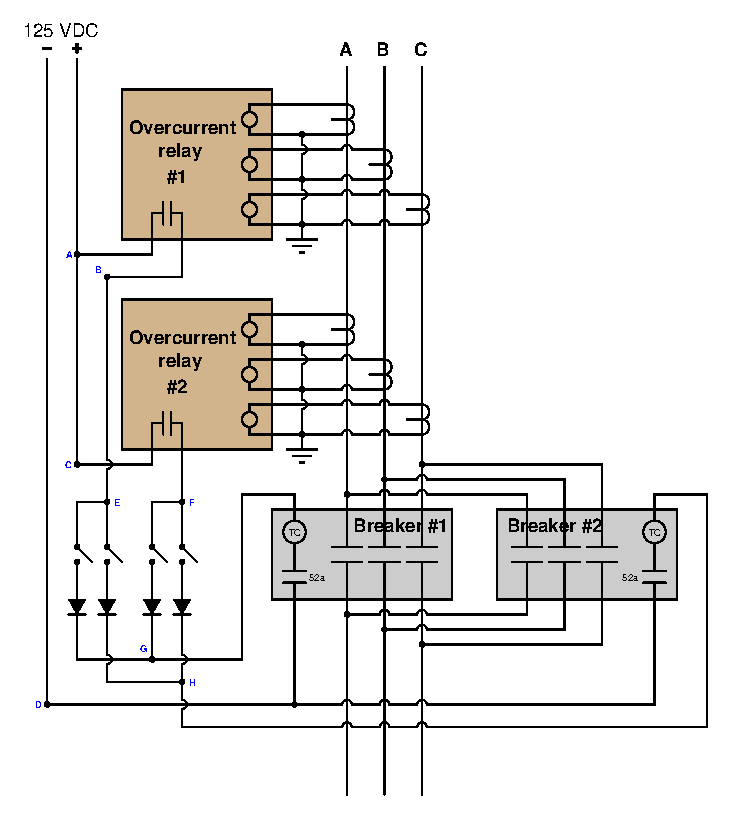
\includegraphics[width=15.5cm]{i02112x04.eps}$$

\vskip 20pt \vbox{\hrule \hbox{\strut \vrule{} {\bf Virtual Trip-testing} \vrule} \hrule}

This question is a good candidate for a ``Virtual Trip-testing'' exercise.  Presenting the diagram to students, you pose an assignment whereby students must figure out how to test some component of this system to check that it will operate as intended to shut down the system in an abnormal (trip) condition, with some realistic limitation (e.g. power cannot be shut off to the load).  Students then propose various methods for executing the test.  Your job is to determine whether or not their proposed tests will achieve the desired result(s).

During and after the exercise, it is good to ask students follow-up questions such as:

\begin{itemize}
\item{} Where might our planned test strategy go wrong?  In other words, what thing(s) might happen to foil our test, either to invalidate the results or to not honor the stated limitation(s)?
\item{} Suppose the limitation were different.  How would this affect our ability to carry out the test?
\item{} Is the last test strategy best one we could execute?
\end{itemize}

%INDEX% Electric power systems: protective relays (time-overcurrent)
%INDEX% Protective relay: time-overcurrent (51)
%INDEX% Safety, shutdown system: trip testing (protective relay circuit)

%(END_NOTES)


